\chapter{The Internet of Things: Components}\label{ch:chapter7}
\section{L'inizio dell'era IOT}
L'Internet del futuro coinvolger� un vastissimo numero di oggetti che useranno uno standard di architettura comune per portare determinati servizi agli utenti. Si prevede infatti che ci saranno decine di miliardi di questi dispositivi interconnessi fra loro nei prossimi anni e questo produrr� nuove interazioni fra il mondo fisico e quello digitale. La risultante di questo paradigma della rete prende il nome di \textit{Internet of Things (IOT} e produrr� un grandissimo numero di opportunit� per gli utenti, per le imprese e per chi fornisce servizi in svariati settori. In particolare le aree che beneficeranno maggiormente dello sviluppo dell'IOT saranno la collezione e l'analisi dei dati, automazioni, incluse nel settore del benessere e del fitness, automazioni per il controllo della casa, per risparmiare energia, per la produzione, per il trasporto, per il controllo ambientale, per lo stoccaggio e la produzione di prodotti, sicurezza e sorveglianza e molto, molto altro ancora.
\newline
Lo sviluppo tecnologico � ancora necessario in molte aree. Infatti negli ultimi anni sono stati condotti molti investimenti in ricerca e sviluppo delle reti wireless. Attualmente la ricerca e lo sviluppo di ricercatori e produttori � indirizzato su protocolli a basso consumo energetico, sicurezza e privacy, protocolli di rete ad alta efficenza energetica per una lunga durata della batteria, affidabilit� delle reti e nodi. Questi sviluppi wireless sono cruciali per la crescita dell'IoT.
\newline
Ci sono altre aree in cui � stato coinvolto lo sviluppo dei devices IoT come ad esempio la capacit� di social networking da parte dei dispositivi, sfruttando comunicazioni \textit{machine-to-machine}, processando e salvando un vastissimo numero di dati in real-time e sviluppando applicazioni che fornissero agli utenti finali interfacce utili e intelligenti per questi dispositivi e dati.

\section{Gli Scopi dell'Internet of Things}
Possiamo fornire le seguenti definizioni per definire gli scopi dell'IoT:
\newline
- \textbf{Internet of Things}: un'infrastruttura globale per le informazioni della societ�, che abilita servizi avanzati grazie all'interconnessione (fisica e virtuale) degli oggetti basandosi su tecnologie e informazioni attualmente esistenti ed in via di sviluppo.
\newline
- \textbf{Thing}: questo � un oggetto del mondo fisico o virtuale capace di essere identificato ed integrato all'interno di reti di comunicazione.
\newline
- \textbf{Device}: � una parte dell'IoT con la capacit� obbligatoria di comunicare e la capacit� opzionale di fare sensing, acuation, salvataggio dei dati e lavorazione di dati.
\newline
\newline

\begin{figure}[htbp]
\centering
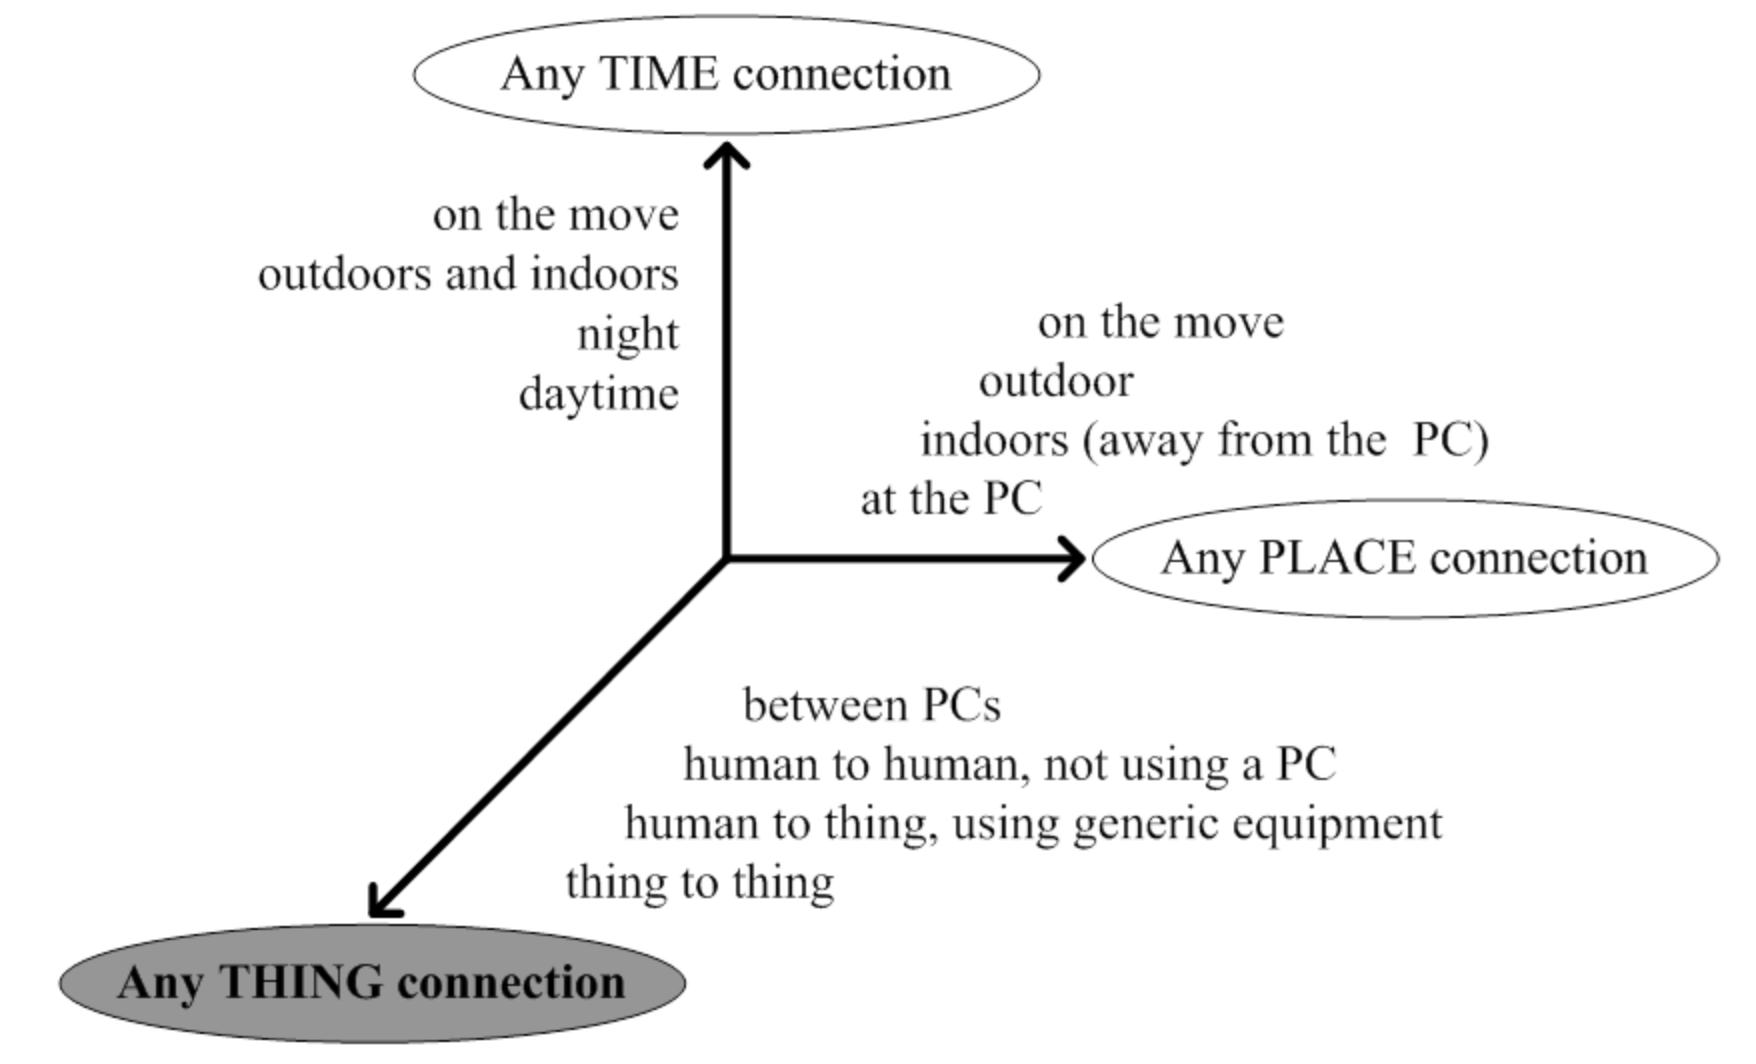
\includegraphics[width=0.80\textwidth,height=\textheight,keepaspectratio]{images/fig_5_8}
\caption{La nuova dimensione introdotta nell'Internet of Things}
\label{fig:5_7}
\end{figure}

L'equazione che pu� riassumere tutto il complesso sistema dell'IoT potrebbe essere la seguente:
\newline
\textit{Oggetti Fisici + Controller, Sensori, Attuatori + Internet} = \textbf{IoT}.

\section{Componenti di oggetti abilitati per l'IoT}
Gli ingredienti chiavi per un sistema di oggetti abilitati all'IoR sono sensori, attuatori, microcontrollers, un mezzo di comunicazione (transceiver) ed un mezzo di identificazione (RFID: radio-frequency identification). Il mezzo di comunicazione � un ingrediente fondamentale senza il quale i dispositivi non potrebbero partecipare in una rete. \cite{machine}

\subsection{Sensori}
Un sensore misura determinati parametri fisici, chimici o biologici e invia un segnale elettronico proporzionato con le caratteristiche rilevate, o in formato digitale oppure sotto forma di un livello di tensione analogico. In entrambi i casi, l'output del sensore � tipicamente l'input di un microcontroller o di un altro elemento di gestione.
\newline
Un sensore pu� operare in \textit{modalit� attiva} quando prende l'iniziativa di inviare i dati rilevati al controller o periodicamente o quando una determinata soglia � superata. Alternativamente il sensore pu� operare in \textit{modalit� passiva} inviando dati solo quando � richiesto dal controller.

\begin{figure}[htbp]
\centering
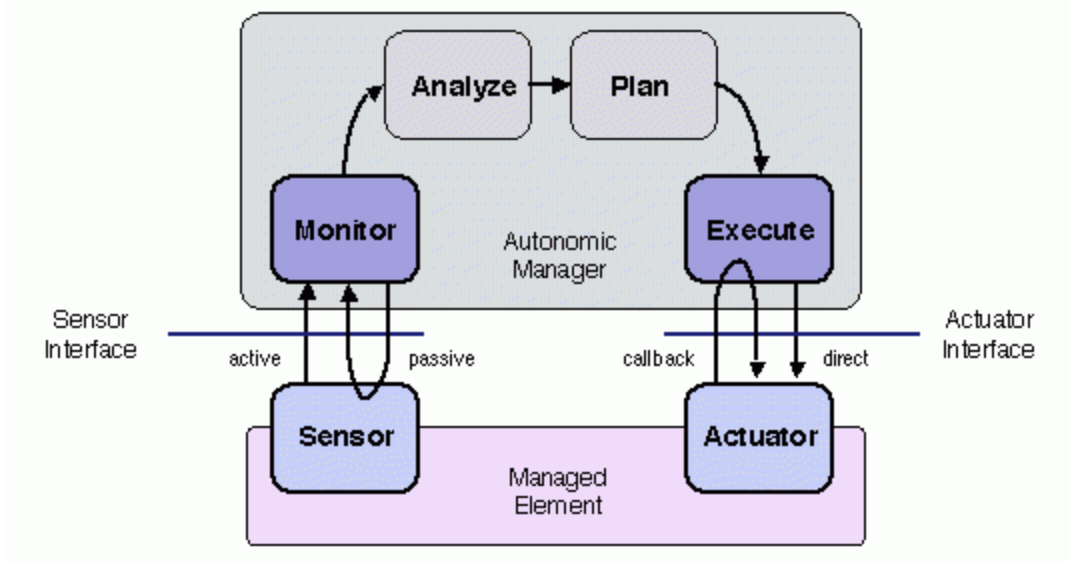
\includegraphics[width=0.80\textwidth,height=\textheight,keepaspectratio]{images/fig_5_9}
\caption{Interfacce per sensori e attuatori}
\label{fig:5_9}
\end{figure}

La tipologie di sensori utilizzati nell'IoT sono moltissime. Ci sono sensori che sono estremamente piccoli, usando nanotecnologie, oppure sensori estremamente grandi come camere di videosorveglianza.
\newline
\newline
Ci sono due concetti chiavi nel distinguere le tipologie di sonsori:
\newline
- \textbf{Accuracy}: si riferisce a quanto una misurazione si avvicina alla verit�. 
\newline
- \textbf{Precision}: si riferisce a quanto sono vicine tra loro pi� misurazioni della stessa quantit� fisica. Collegata con questo concetto troviamo la \textbf{Resolution}, ovvero la qualit� dell'output del sensore.
\newline
Se un sensore ha bassa accuracy, questo produce un errore sistematico. Se un sensore ha bassa precucione, produce un errore di riproducibilit�.

\subsection{Attuatori}
Un attuatore riceve un segnale elettronico dal controller e risponde interagendo con l'ambiente per produrre un effetto su qualche parametro fisico, biologico o chimico di una determinata entit�. 
\newline
Nella modalit� di operazione \textit{direct mode}, il controller invia un segnale che attiva gli attuatori. Invece nella \textit{callback mode} gli attuatori rispondono al controller per riportare un completamento o un problema e richiedono ulteriori istruzioni. 
\newline
\newline
Gli attuatori sono generalmenti classificati come segue:
\newline
- \textbf{Idraulici}: sono costituiti da un cilindro o un motore fluido che utilizza la forza idraulica per facilitare processi meccanici.
\newline
- \textbf{Pneumatici}: lavorano come quelli idraulici solo che utilizzano gas al posto di liquido.
\newline
- \textbf{Elettrici}: sono dispositivi alimentati da motori che convertono l'energia elettrica in coppia meccanica. 
\newline
- \textbf{Meccanici}: funzionano mediante movimento rotazionale o lineare e sono utilizzati per convertire il movimento. 

\subsection{Microcontrollers}
La cosa smart nei dispositivi che si definisco tali � fornita da un microprocessore perfettamente integrato. Adesso vedremo alcuni termini chiave per esplicare il concetto di microcontroller.
\newline
\textbf{Embedded System}
\newline
Il termine \textit{embedded system} si riferisce all'uso di elettronica e di software all'interno di un dispositivo che ha una o pi� funzioni.
\newline
\textbf{Application Processors vs Dedicated Processor}
\newline
\textit{Application processor} sono definiti dall'abilit� del processore di eseguire complessi sistemi operativi. Un classico esempio dell'uso di embedded application processor � lo smartphone, poich� � designato ad usare svariate applicazioni e svolgere molte funzioni diverse.
\newline
La maggior parte degli embedded systems utilizza un \textit{dedicated processor}, il quale � dedicato ad una o ad un piccolo numero di specifiche funzionalit� richieste dall'host. 
\newline
\textbf{Microprocessors}
\newline
Un processore i cui elementi sono stati miniaturizzati in un unico o in pi� circuiti integrati.
\newline
\textbf{Microcontrollers}
\newline
Un singolo chip che contiene il processore, la memoria non volatile (ROM), la memoria volatile per input/output (RAM), un clock ed una unit� di controllo I/O. Il loro impiego � fondamentale per utilizzare in maniera sostanzialmente differente lo spazio logico sul disponibile. 
\newline
\textbf{Deeply Embedded System}
\newline
� un sottoinsieme degli embedded system e possiamo dire che ha un processore il cui comportamento � difficile da osservare sia da parte del programmatore che dall'utente. Un deeply embedded system utilizza un microcontrollor, non � programmabile una volta che la logica del programma per il dispositivo � stata scritta nella ROM e non ha nessuna interazione con l'utente.

\subsection{Transceivers}
Un transceiver contiene i componenti elettronici necessari per ricevere e trasmettere dati. La maggior parte dei dispositivi IoT contiene un transceiver wireless, capace di comunicare utilizzando la Wi-Fi, ZigBee ed altri schemi wireless. 

\subsection{RFID}
La tecnologia Radio-frequency identification (RFID) utilizza onde radio per identificare oggetti e sta diventando una tecnologia che facilita sempre di pi� l'IoT.
\newline
Gli elementi principali per un sistema RFID sono i \textit{tags} ed i \textit{readers}. 
\newline
I \textit{tags} sono piccoli oggetti programmabili usati per il monitoraggio di oggetti, animali ed esseri umani. Sono disponibili in varie forme, dimensioni, funzionalit� e costi. 
\newline
I \textit{readers} acquisiscono e qualche volta riscrivono le informazioni salvate sui tags che rientrano nel loro raggio di azione. 

\begin{figure}[htbp]
\centering
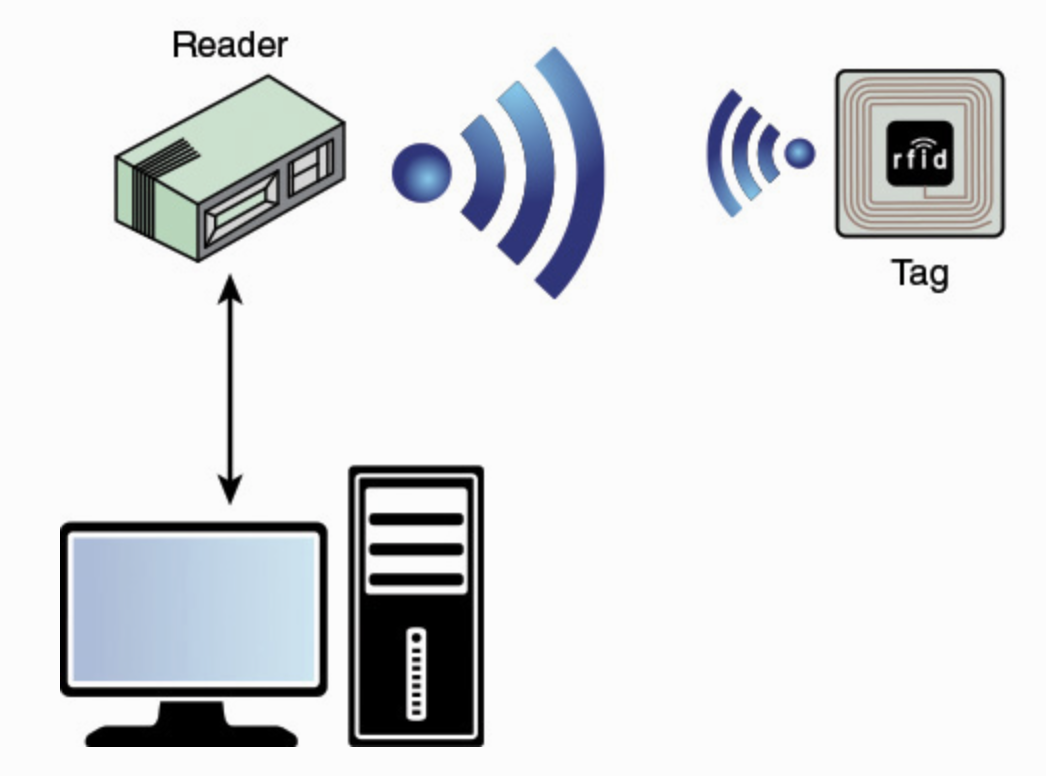
\includegraphics[width=0.80\textwidth,height=\textheight,keepaspectratio]{images/fig_5_10}
\caption{Elementi di un sistema RFID}
\label{fig:5_9}
\end{figure}
